%!TEX root = ../../schlussbericht.tex
\chapter{Zielerreichung}
	
	
	\section{Erfüllung der Requirements}	
	Wir konnten unser Projekt fertigstellen und somit unser Ziel erreichen. Die von uns gestellten Anforderungen in der Anforderungsspezifikation konnten erfüllt werden.
	
	\begin{table}[H]
        \tablestyle
        \tablealtcolored
        \begin{tabularx}{\textwidth}{X X}
        \tableheadcolor
            \tablehead Funktion & 
            \tablehead Ort \\  
        \tablebody
            \textbf{F01} Planung der Helfereinsätze & 
            /Event/Edit/\{id\}  \tabularnewline
            
            \textbf{F02} Unterteilung des Einsatz nach Zeit und Funktion & 
            /Event/Edit/\{id\}  \tabularnewline
            
             \textbf{F03} Importieren der Spieldaten von Webservice & 
            /EventImport  \tabularnewline
            
              \textbf{F04} Manuelles Erfassen von Spieldaten & 
            /Event/Create  \tabularnewline
            
              \textbf{F05} Importieren der Endbenutzer aus webling.ch & 
            /MemberImport  \tabularnewline
            
              \textbf{F06} Manuelles Erfassen von Mitglied & 
            /Account/Create  \tabularnewline
            
              \textbf{F07} Einteilung der Einsätze nach Mannschaft & 
            /Event/Edit/\{id\}  \tabularnewline
            
            \textbf{F08} Einschreiben eines Mitglieds für Einsatz & 
            /Event/Details/\{id\} \newline /HelperTask/Details/\{id\}  \tabularnewline
            
            \textbf{F09} Austragen eines Mitglieds von Einsatz innerhalb Frist & 
            /Event/Details/\{id\} \newline /HelperTask/Details/\{id\}  \tabularnewline
            
            
            \textbf{F10} Übersicht der Einsätze für Mitglied & 
            \textit{Startseite}  \tabularnewline
            
            \textbf{F11} Erinnerung der Helfer vor Einsatz via E-Mail & 
            -  \tabularnewline
            
        \tableend
        
        \end{tabularx} 
    \end{table}
	
	\section{Nicht realisierte Features}
	
    \newpage
	\section{Kosten und Zeit}	
        \begin{wrapfigure}[14]{R}{0.7\textwidth}
            \vspace{-25pt}
            \begin{center}
                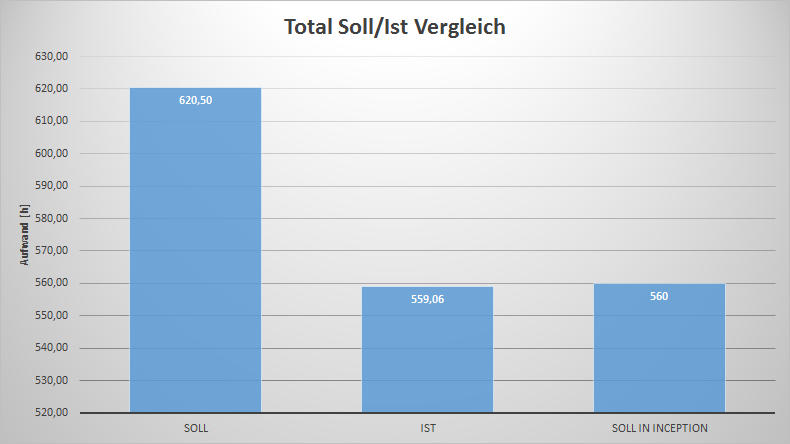
\includegraphics[width=0.7\textwidth]{content/schlussbericht/images/zeit_total_schaetzung.png}
            \end{center}
            \vspace{-20pt}
            \caption{Total Soll/Ist Vergleich}
        \end{wrapfigure}
        Wir haben von Anfang an sehr defensive Schätzungen gemacht. Mit der Projektvorgabe von 10 Stunden/Woche (vgl. \enquote{Soll in Inception}) haben wir uns einen zusätzlichen Puffer ermöglicht, um auf Risiken reagieren zu können.
        \\ Einzig in der Inception-Phase haben wir eine grössere Ist-Zeit als geschätzt gehabt. Für die nachfolgenden Phasen wurde die Soll-Zeit mind. eingehalten oder gar unterboten. 
        \vspace{1cm}

	\section{Aufwand nach Phase}
        \begin{wrapfigure}[15]{L}{0.7\textwidth}
            \vspace{-25pt}
            \begin{center}
                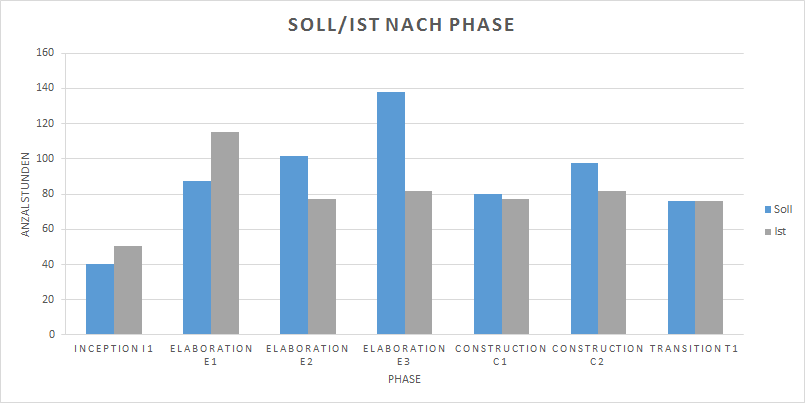
\includegraphics[width=0.7\textwidth]{content/schlussbericht/images/zeit_nach_phase.png}
            \end{center}
            \vspace{-20pt}
            \caption{Soll/Ist nach Phase}
        \end{wrapfigure}
        Die Phase Elaboration E3 war während der Inception Phase nicht geplant. Der Stand nach E2 war schlicht noch zu wenig konkret, sodass wir uns im Gespräch mit dem Betreuer für eine zusätzliche Elaboration Phase entschieden haben. Es wurden dann viele konkrete Kern-Issues in die Phase aufgenommen, sodass die Soll-Zeit für \enquote{Elaboration E3} entsprechend hoch war. Durch die sehr gute Vorarbeit resp. Softwarearchitektur konnten die Issues aber massiv schneller umgesetzt werden, als geplan. Daher entstand alleine für \enquote{Elaboration E3} eine zeitliche Differenz von ca. 50h.
	
    \newpage
	\section{Aufwand pro Person}
        \begin{wrapfigure}[8]{R}{0.7\textwidth}
            \vspace{-25pt}
            \begin{center}
                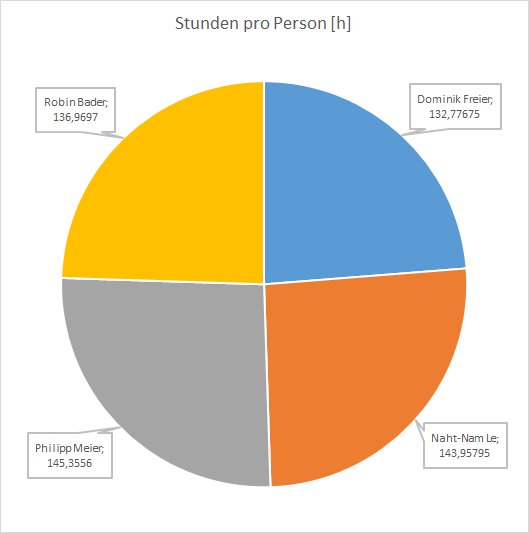
\includegraphics[width=0.7\textwidth]{content/schlussbericht/images/zeit_nach_person.png}
            \end{center}
            \vspace{-20pt}
            \caption{Stunden pro Person}
        \end{wrapfigure}
        Für uns war es wichtig, eine möglichst grosse Ausgewogenheit der Aufwände über alle Team-Mitglieder zu erzielen. Dieses Ziel wurde für jede Phase verfolgt und am Schluss resultierte ein knappes Delta von ca. 8 Stunden.
        \vspace{4cm}
	
	\section{Anz. Code-Commits im zeitlichen Verlauf}
        \begin{wrapfigure}[8]{L}{0.7\textwidth}
            \vspace{-25pt}
            \begin{center}
                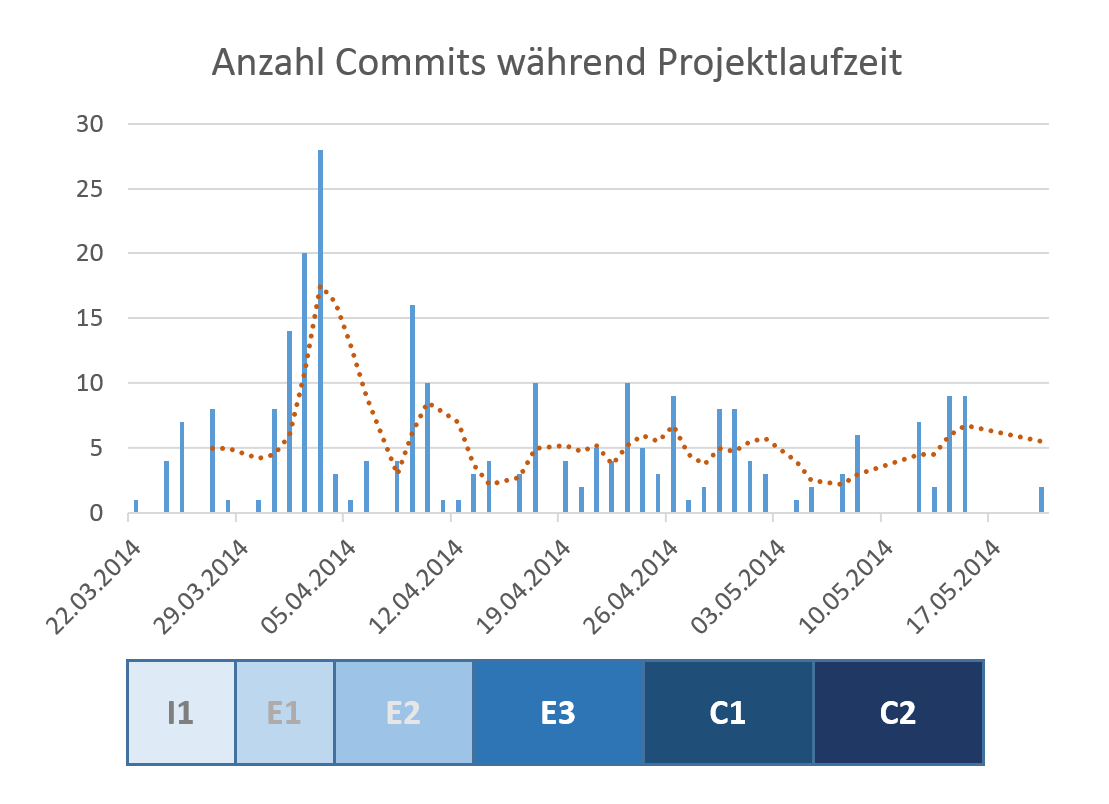
\includegraphics[width=0.7\textwidth]{content/schlussbericht/images/commitspertime.png}
            \end{center}
            \vspace{-20pt}
            \caption{Anz. Commits auf Zeitstrahl}
        \end{wrapfigure}
        Wie in SE1 gelernt, entsteht ein erheblicher Teil des Projekts bereits während den Elaboration-Phasen. In unserem Projekt waren  knapp 2/3 während der Inception und Elaboration Phasen.

	